%==============================================================================
% Sjabloon poster bachproef
%==============================================================================
% Gebaseerd op document class `a0poster' door Gerlinde Kettl en Matthias Weiser
% Aangepast voor gebruik aan HOGENT door Jens Buysse en Bert Van Vreckem

\documentclass[a0,portrait]{hogent-poster}

% Info over de opleiding
\course{Graduaatsproef}
\studyprogramme{Graduaat in het Programmeren}
\academicyear{2024-2025}
\institution{Hogeschool Gent, Valentin Vaerwyckweg 1, 9000 Gent}

% Info over de bachelorproef
\title{Cross platform application with Vue,\newline Quasar and NestJS}
\subtitle{Advantages and challenges of a single source codebase}
\author{Rafal Kowalski}
\email{rafal.kowalski@student.hogent.be}
\supervisor{Luc Vervoort (HoGent)}
% \cosupervisor{Wim Goedertier (HoGent)}

% Indien ingevuld, wordt deze informatie toegevoegd aan het einde van de
% abstract. Zet in commentaar als je dit niet wilt.
\specialisation{Programmeren}
\keywords{Vue, Quasar, NestJs, Electron, Cordova}
\projectrepo{https://github.com/rafalhogent/medikohogent}

\begin{document}

\maketitle

\begin{abstract}

  Cross-platform ontwikkeling biedt vele mogelijkheden voor programmeurs, waarbij één enkele codebase wordt tegelijkertijd omgezet in toepassingen die werken op meerdere verschillende platformen. De graduaatsproef zal proberen antwoord te geven op de vraag of de softwareontwikkelingsmethode op basis van het gebruik van één broncode en publicatie op vele platformen effectief betrouwbaar werkende applicatie kan leveren. Die methode kan zeer nuttig zijn voor programmeurs die hun code als standalone applicatie ook willen publiceren. De literatuurstudie helpt om beschikbare oplossingen te vergelijken en om de keuze van de frameworks voor de proof-of-concept-applicatie te rechtvaardigen. \newline
  Het project is geschreven in één programmeertaal en geïmplementeerd op verschillende apparaten met één codebase. Er wordt ook een strategie voorgesteld om gebruikersdata te synchroniseren tussen alle frontend-clients.
  Ten slotte worden de resultaten geëvalueerd. De moeilijkheden tijdens het ontwikkelingsproces worden benadrukt. De prestaties en stabiliteit van de applicaties worden geanalyseerd, en de grootte van de builds wordt vergeleken.
\end{abstract}

\begin{multicols}{2} % This is how many columns your poster will be broken into, a portrait poster is generally split into 2 columns

\section{Introductie}

Het ontwikkelen van een applicatie vereist vaak veel kennis en ervaring, werken met meerdere talen kan een extra moeilijkheid zijn.
De motivatie voor het schrijven van deze thesis is om een eenvoudige en efficiënte methode te ontwikkelen voor het coderen en publiceren van cross-platform applicaties die beschikbaar zijn op alle populaire en veelgebruikte apparaten.\newline

De graduaatsproef onderzoeksvraag:
\textbf{Welke voordelen en moeilijkheden kunnen we verwachten bij het maken van applicaties voor meerdere platformen met gebruik maken van één enkele codebron in JS/TS, het Quasar-framework, Electron en Cordova? }

Het doel van deze thesis is om een collectie van proof-of-concept client-applicaties te bouwen voor verschillende besturingssystemen en web-browsers die gebruikersdata via een server kunnen synchroniseren.

\section{Methodologie}
Het onderzoek is uitgevoerd door de analyse van bestaande cross-platform oplossingen en door het maken van een Proof-of-Concept applicatie. Graduaatsproef als applicatieontwikkeling is een taak die niet alleen kennis van programmeertalen vereist, maar ook technische vaardigheden, dus het kan alleen worden gemaakt door mensen met IT-achtergrond. De thesis bestaat uit onderstaande werkfasen:
\begin{itemize}
    \item onderzoek van beschikbare cross-platform oplossingen
    \item ontwikkelen van een proof-of-concept-applicatie, inclusief lay-out, domein en architectuurontwerp, implementatie van functionaliteiten
    \item implementatie van synchronisatie via server
    \item builds voor verschillende besturingssystemen en web
    \item analyse van resultaten, voordelen en moeilijkheden
\end{itemize}

\section{Proof-of-Concept}
Om de grootste flexibiliteit te bereiken, werd er een client-server architectuur gebruikt. Een van de grootste voordelen van deze oplossing is de mogelijkheid om gegevens te delen met verschillende gebruikers of verschillende apparaten van dezelfde gebruiker. De client (Quasar \& Vue) is gepubliceerd als web-applicatie (SPA), Linux \& Windows Desktop (Electron) en mobile (Cordova).

De bedoeling was om de applicatie volledig in de offline modus te laten werken en de lokaal opgeslagen gegevens te synchroniseren met de cloudserver (NestJs), op aanvraag van de gebruiker of automatisch op de achtergrond.

\begin{center}
  \captionsetup{type=figure}
  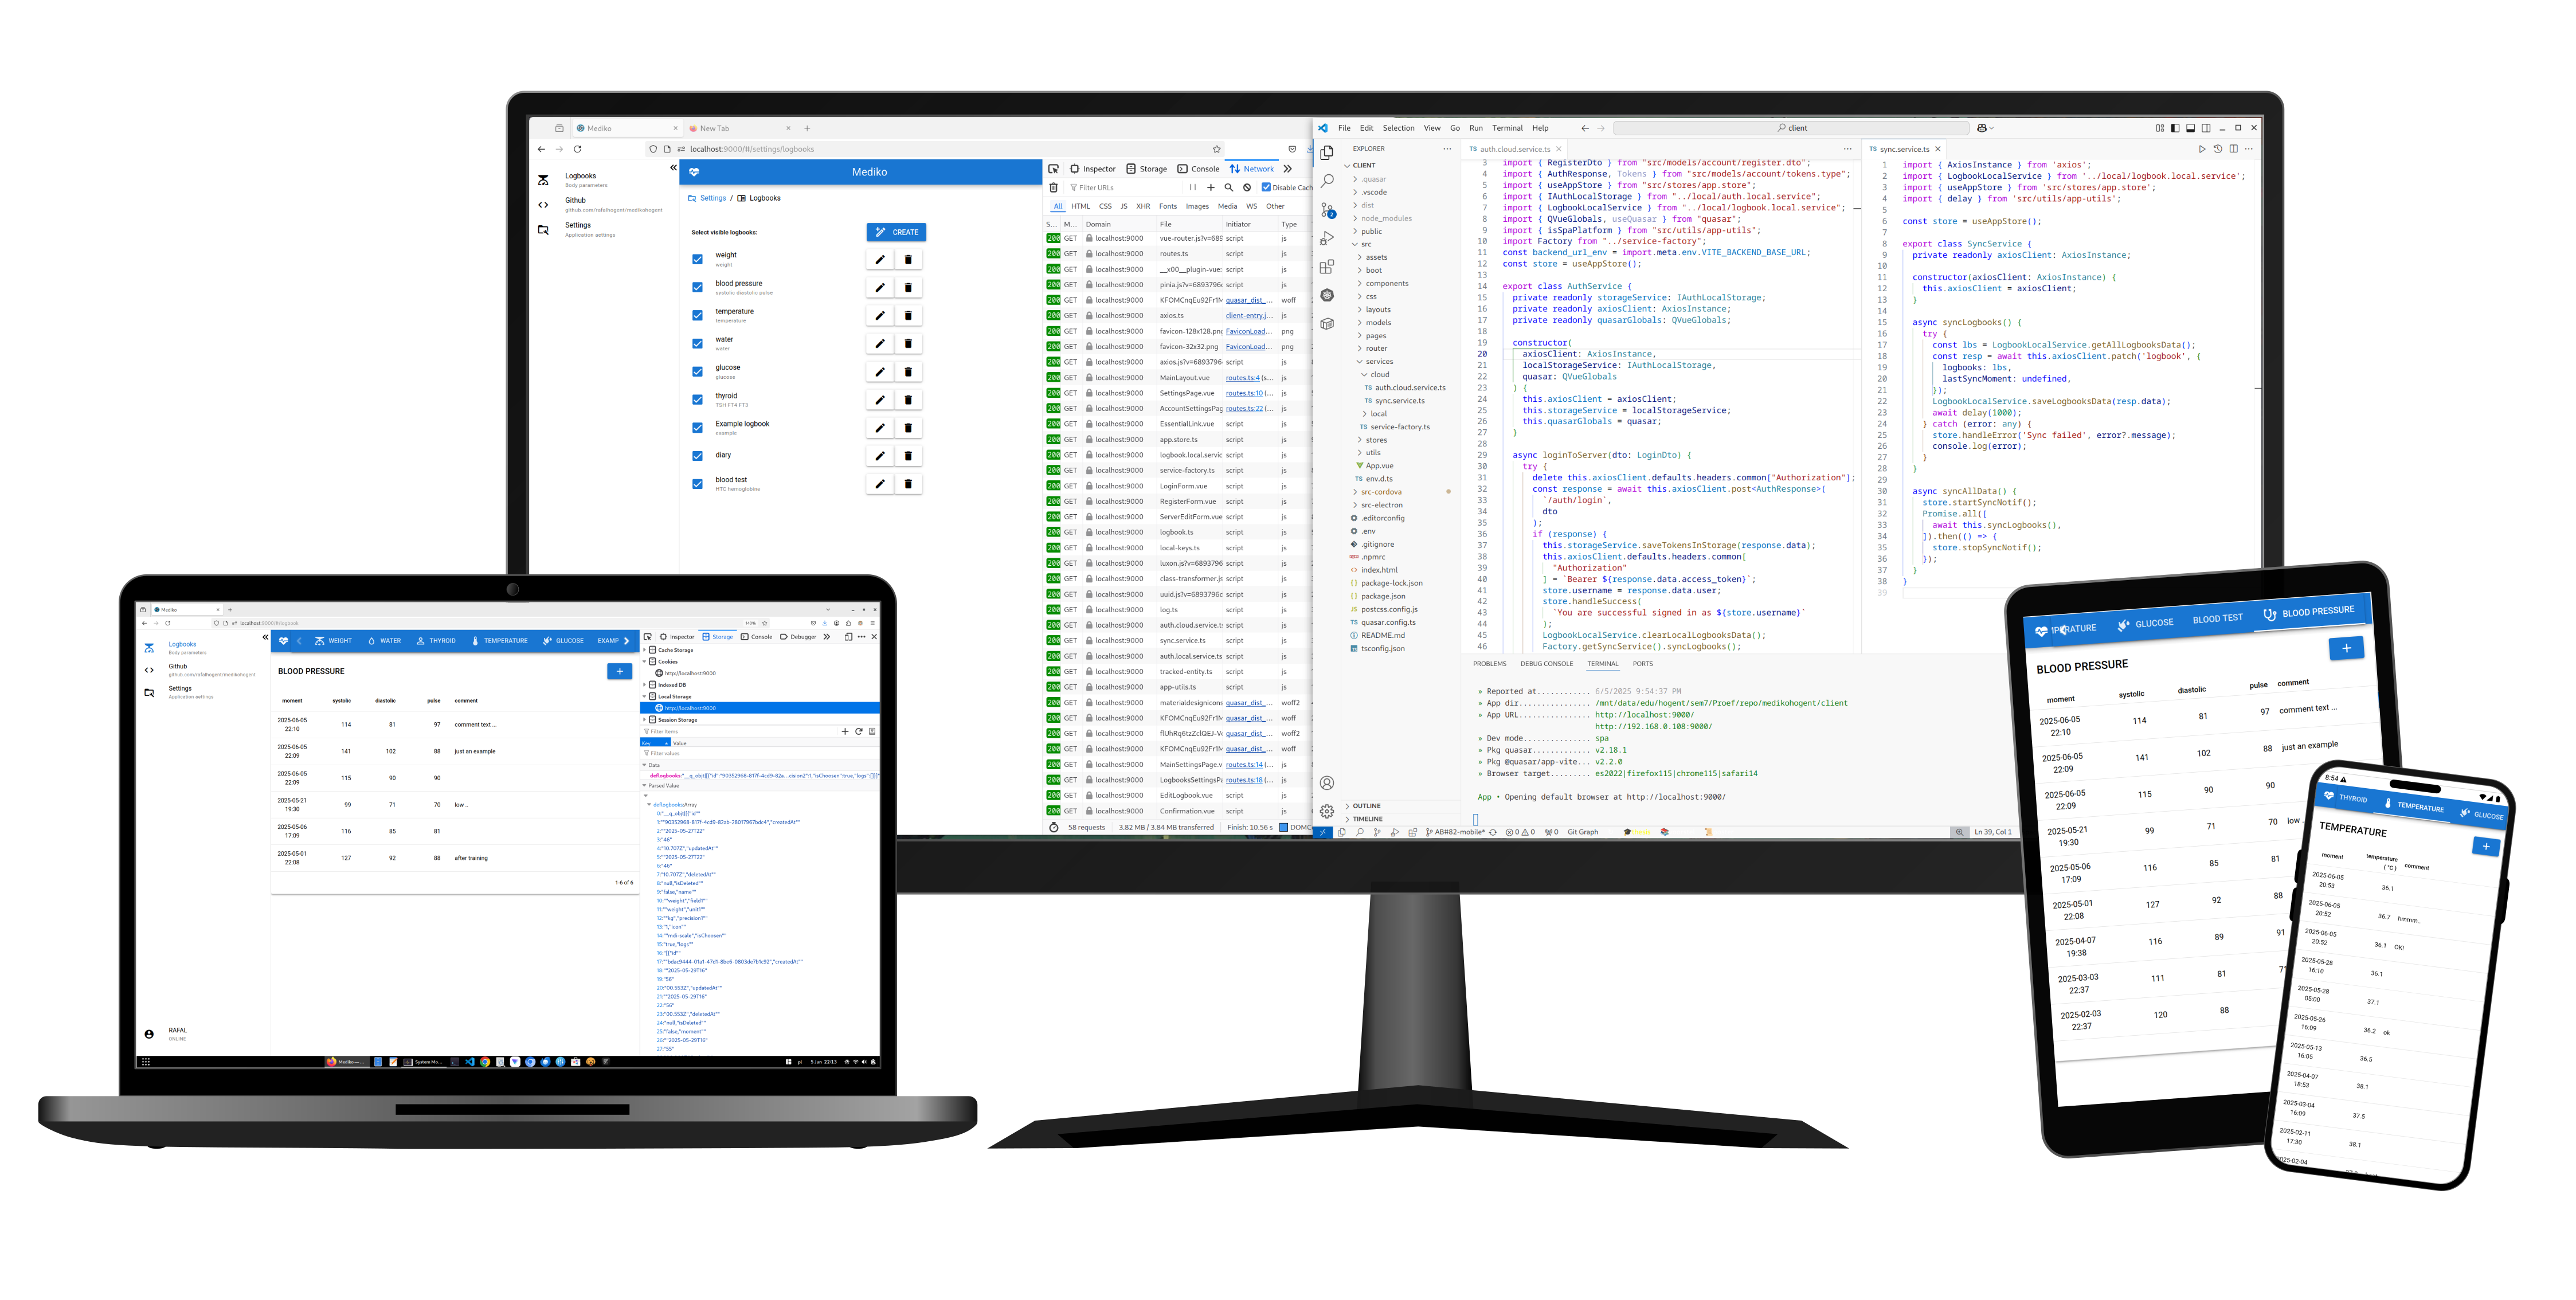
\includegraphics[width=1.0\linewidth]{responsive}
  \captionof{figure}{Cross platform Applicatie met Quasar \& Vue.JS  }
\end{center}



\section{Conclusies}

Deze thesis heeft een sjabloon gepresenteerd voor het ontwerp en de implementatie van een webgebaseerde platformonafhankelijke applicatie-ontwikkeling. De kwaliteit van de geleverde template is consistent met verwachtingen. Ondanks enkele problemen was het schrijven van de code en het maken van builds voor verschillende toestellen geen moeilijke taak, in plaats daarvan leverde het interessante ervaring en kans om de technologie beter te kennen.

De grootste moeilijkheden zijn onder meer:
\begin{itemize}
    \item conflicten bij het bouwen met verschillende technologieën
    \item consistente gebruikersinterface onderhouden op alle platforms
    \item beperkte prestaties en moeilijke optimalisatie in vergelijking met native frameworks
\end{itemize}


De grootste voordelen:
\begin{itemize}
    \item versneld ontwikkelingsproces
    \item gemakkelijkere gebruikersinterface harmonisatie
    \item snellere implementatie van wijzigingen op alle platforms tegelijkertijd
    \item gecentraliseerde broncode

\end{itemize}

\section{Toekomstig onderzoek}

\begin{itemize}
    \item prestatietests onder hoge belasting met veel gegevens
    \item code delen tussen client en server
    \item builds voor Apple-toestellen
    \item implementatie van p-o-c met gebruik van andere cross-platform frameworks
\end{itemize}

\end{multicols}
\end{document}